% !TeX root = surprises.tex

\chapter{Sind Dreiecke mit gleichen Flächen und Umfängen kongruent?}\label{c.congruent}

%%%%%%%%%%%%%%%%%%%%%%%%%%%%%%%%%%%%%%%%%%%%%%%%%%%%%%%%%%%%%%%

Sind zwei Dreiecke mit der gleichen Fläche und dem gleichen Umfang kongruent? Nicht unbedingt:  Die Dreiecke mit den Seiten $(17,25,28)$ und $(20,21,29)$ haben beide einen Umfang von $70$ und einen Flächeninhalt von $210$, sind aber nicht kongruent (Abb.~\ref{f.congruent-first-example}). \footnote{Die Flächen wurden mit Hilfe der Heronschen Formel (Thm.~\ref{thm.heron}) und die Winkel mit Hilfe des Kosinussatzes (Thm.~\ref{thm.law-of-cosines}) berechnet.} In diesem Kapitel wird gezeigt, dass es bei einem Dreieck mit rationalen Seiten möglich ist, ein nicht kongruentes Dreieck mit ebenfalls rationalen Seiten zu konstruieren, das denselben Flächeninhalt und Umfang hat.
Wir führen die Herleitung anhand eines Beispiels durch und zeigen, dass das Dreieck mit den Seiten $(3,4,5)$ und das Dreieck mit den Seiten 
$\left(\frac{156}{35}, \frac{101}{21}, \frac{41}{15}\right)$ beide einen Umfang $12$ und einen Flächeninhalt $6$ haben.

\begin{figure}[b]
\begin{center}
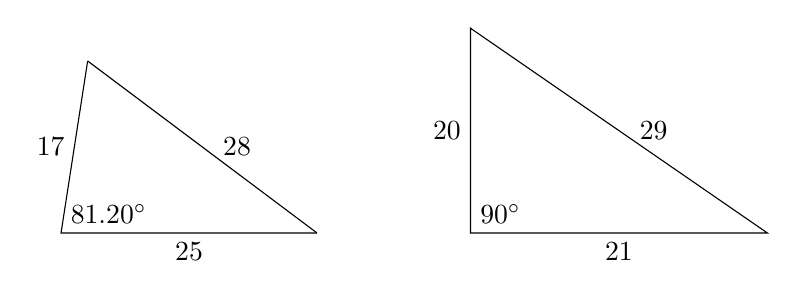
\begin{tikzpicture}[scale=1.3]
\coordinate (A1) at (0,0);
\node[above right] at (A1) {$81.20^\circ$};
\coordinate (B1) at (2.5cm,0);
\coordinate (C1) at (81.20:1.7cm);
\draw (B1) -- node[below] {$25$} (A1) -- node[left] {$17$} (C1);
\draw (B1) -- node[right,xshift=4pt] {$28$} +(143.13:2.8cm);
\begin{scope}[xshift=4cm]
\coordinate (A2) at (0,0);
\node[above right] at (A2) {$90^\circ$};
\coordinate (B2) at (2.9cm,0);
\coordinate (C2) at (0,2cm);
\draw (B2) -- node[below] {$21$} (A2) -- node[left] {$20$} (C2) -- node[right,xshift=4pt] {$29$} cycle;
\end{scope}
\end{tikzpicture}
\end{center}
\caption{Nicht kongruente Dreiecke mit gleicher Fläche und gleichem Umfang}\label{f.congruent-first-example}
\end{figure}


\section{Von einem Dreieck zu einer elliptischen Kurve}\label{s.elliptic}

Die drei Winkelhalbierenden eines Dreiecks schneiden sich in einem Punkt, der als \emph{incenter} des Dreiecks bezeichnet wird. Der Mittelpunkt ist der Mittelpunkt eines in das Dreieck einbeschriebenen Kreises (Abb.~\ref{f.congruent1}). 

Ziehe vom Mittelpunkt $O$ aus Höhenlinien zu den Seiten. Die Höhen haben die Länge $r$, den Radius des Inkreises. Die Höhen und Winkelhalbierenden bilden drei Paare von kongruenten rechtwinkligen Dreiecken:
\[
\triangle AOB'\cong \triangle AOC',\quad \triangle BOA'\cong \triangle BOC',\quad \triangle COA'\cong \triangle COB'\,.
\]

\begin{figure}[t]
\begin{center}
\begin{tikzpicture}[scale=1.85]
% Draw base and path two lines at known angles
\draw (0,0) coordinate (a) node[below] {$A$} --
  (0:6) coordinate (b) node[below] {$B$};
\path[name path=ac] (a) -- +(50:4);
\path[name path=bc] (b) -- +(150:5);
% Get their intersection and draw lines between vertices
\path[name intersections={of=ac and bc,by=c}];
\node[above] at (c) {$C$};
\draw (a) -- (c) -- (b) -- (a);
% Label angles with tick marks
\draw (a) ++(0:4mm) arc (0:50:4mm);
\draw (a) ++(10:3.5mm) -- +(10:1mm);
\draw (a) ++(15:3.5mm) -- +(15:1mm);
\draw (a) ++(35:3.5mm) -- +(35:1mm);
\draw (a) ++(40:3.5mm) -- +(45:1mm);
\draw (b) ++(150:5mm) arc (150:180:5mm);
\draw (b) ++(157.5:4.5mm) -- +(157.5:1mm);
\draw (b) ++(172.5:4.5mm) -- +(172.5:1mm);
\draw (c) ++(230:3mm) arc (230:330:3mm);
\draw (c) ++(250:2.5mm) -- +(250:1mm);
\draw (c) ++(255:2.5mm) -- +(255:1mm);
\draw (c) ++(260:2.5mm) -- +(260:1mm);
\draw (c) ++(300:2.5mm) -- +(300:1mm);
\draw (c) ++(305:2.5mm) -- +(305:1mm);
\draw (c) ++(310:2.5mm) -- +(310:1mm);
% Path bisectors of two lines
\path[name path=bia] (a) -- +(25:3.5);
\path[name path=bib] (b) -- +(165:5);
% Intersection of angle bisectors
\path [name intersections={of=bia and bib,by=center}];
% Draw angle bisectors to center
\draw (a) -- (center);
\draw (c) -- (center);
\draw (b) -- (center);
% Draw radii
\draw (center) -- node[left] {$r$}
  ($(a)!(center)!(b)$) node[below,yshift=-2pt] {$C'$}
  coordinate (ap);
\draw (center) -- node[left,yshift=-4pt] {$r$}
  ($(a)!(center)!(c)$) node[above left,xshift=4pt] {$B'$}
  coordinate (bp);
\draw (center) -- node[right] {$r$}
  ($(b)!(center)!(c)$) node[above right] {$A'$}
  coordinate (cp);
\vertex{center};
\node[above,xshift=3pt,yshift=6pt] at (center) {$O$};
% Draw right angle squares
\draw (ap) rectangle +(3pt,3pt);
\draw[rotate=-40] (bp) rectangle +(3pt,3pt);
\draw[rotate=-120] (cp) rectangle +(3pt,3pt);
% Labels of angles
\node[above,xshift=5pt,yshift=21pt]
  at (center) {$\gamma/2$};
\node[above left,xshift=-4pt,yshift=21pt]
  at (center) {$\gamma/2$};
\node[above right,xshift=4pt,yshift=-5pt]
  at (center) {$\beta/2$};
\node[below right,yshift=-6pt]
  at (center) {$\beta/2$};
\node[left,xshift=-8pt,yshift=3pt]
  at (center) {$\alpha/2$};
\node[below left,xshift=2pt,yshift=-6pt]
  at (center) {$\alpha/2$};
% Labels of line segments (names of points are weird...)
\path (a) -- node[below,yshift=-2pt] {$u$} (ap);
\path (a) -- node[left, xshift=-2pt] {$u$} (bp);
\path (b) -- node[above,yshift=2pt]  {$v$} (cp);
\path (b) -- node[below,xshift=-2pt] {$v$} (ap);
\path (c) -- node[above,xshift=-2pt] {$w$} (bp);
\path (c) -- node[above,xshift=2pt]  {$w$} (cp);
% Labels of sides
\draw[<->] ($(a)+(0,-10pt)$) -- node[fill=white] {$c$} 
           ($(b)+(0,-10pt)$);
\draw[<->] ($(a)+(-4pt,7pt)$) -- node[fill=white] {$b$}
           ($(c)+(-4pt,7pt)$);
\draw[<->] ($(b)+(2pt,9pt)$) -- node[fill=white] {$a$}
           ($(c)+(2pt,9pt)$);
% Inscribed circle
\node[draw,circle through=(ap)] at (center) {};
\end{tikzpicture}
\end{center}
\caption{Ein Kreis, der in ein Dreieck eingeschrieben ist}\label{f.congruent1}
\end{figure}

Die Höhen unterteilen die Seiten $a,b,c$ in die Segmente $u,v,w$. Der Flächeninhalt des $\triangle ABC$ ist die Summe der Flächeninhalte von $\triangle BOC, \triangle AOB, \triangle AOC$:
\begin{subeqnarray}
A &=& \frac{1}{2}(w+v)r + \frac{1}{2}(v+u)r + \frac{1}{2}(u+w)r\\
&=&\frac{1}{2}\cdot 2(u+v+w)r\\
&=&\frac{1}{2}(a+b+c)r\\
&=&sr\,, \slabel{eq.area1}
\end{subeqnarray}
Dabei ist $s$ der \emph{Halbumfang}, die Hälfte des Umfangs des Dreiecks $\triangle ABC$. Die Längen von $u,v,w$ können durch den Radius des Kreises und die zentralen Winkel $\alpha/2,\beta/2,\gamma/2$ ausgedrückt werden:
\begin{align}
\tan \frac{\alpha}{2}= \frac{u}{r},\quad
\tan \frac{\beta}{2} = \frac{v}{r},\quad
\tan \frac{\gamma}{2} =\frac{w}{r}\,.\label{eq.uvw}
\end{align}
Der Halbumfang kann nun durch die Tangenten ausgedrückt werden:
\[
s = u+v+w = r\tan \frac{\alpha}{2}+r\tan \frac{\beta}{2}+r\tan \frac{\gamma}{2} = r\left(\tan \frac{\alpha}{2}+\tan \frac{\beta}{2}+\tan \frac{\gamma}{2}\right)\,,
\]
und nach Gl.~\ref{eq.area1} ist die Fläche:
\begin{align}
A = sr = r^2\left(\tan \frac{\alpha}{2}+\tan \frac{\beta}{2}+\tan \frac{\gamma}{2}\right)\,.\label{eq.area2}
\end{align}
Aus $r=A/s$ lässt sich Gl.~\ref{eq.area2} wie folgt schreiben:
\begin{align}
\tan \frac{\alpha}{2}+\tan \frac{\beta}{2}+\tan \frac{\gamma}{2} = \frac{A}{r^2} = \frac{A}{(A/s)^2} = \frac{s^2}{A}\,.\label{eq.area3}
\end{align}
Da die Summe der Winkel $\alpha,\beta,\gamma$ $360^\circ$ beträgt:
\begin{subeqnarray}
\gamma/2 &=& 360^\circ/2 - (\alpha/2 + \beta/2)\\
\tan\gamma/2 &=& \tan(180^\circ - (\alpha/2 + \beta/2))\\
 &=& -\tan (\alpha/2 + \beta/2)\\
&=& \frac{\tan\alpha/2 + \tan\beta/2}{\tan\alpha/2 \, \tan\beta/2-1}\,,\slabel{eq.tangent1}
\end{subeqnarray}
mit Hilfe der Formel für den Tangens der Summe von zwei Winkeln (Thm.~\ref{thm.tangent-sum}).

Wir vereinfachen die Notation, indem wir Variablen für die Tangens definieren:
\begin{align}
x=\tan \frac{\alpha}{2},\quad
y=\tan \frac{\beta}{2},\quad
z=\tan \frac{\gamma}{2}\,.\label{eq.variables-for-tangents}
\end{align}
Durch Gl.~\ref{eq.tangent1} können wir $z=\tan\gamma/2$ in Form von $x,y$ ausdrücken:
\begin{align}
z = \frac{x+y}{xy-1}\,.\label{eq.xy1}
\end{align}
Mit dieser Schreibweise wird aus Gl.~\ref{eq.area3}:
\begin{align}
x+y+\frac{x+y}{xy-1}=\frac{s^2}{A}\,.\label{eq.xy2}
\end{align}
Gibt es bei festen Werten von $A$ und $s$ mehrere Lösungen von Gl.~\ref{eq.xy2}?

Für das rechtwinklige Dreieck $(3,4,5)$:
\begin{align}
\frac{s^2}{A} = \frac{\left(\frac{1}{2}(3+4+5)\right)^2}{\frac{1}{2}\cdot 3\cdot 4} = \frac{6^2}{6}=6\,.
\end{align}
\noindent{}Gibt es eine weitere Lösung Gl.~\ref{eq.xy2} mit $s^2/A=6$, so kann sie wie folgt geschrieben werden:
\begin{subeqnarray}
x+y+\frac{x+y}{xy-1}&=&6\\
x^2y + xy^2 -6xy + 6 &=& 0\,.\slabel{eq.elliptic}
\end{subeqnarray}
Dies ist eine Gleichung für eine \emph{elliptische Kurve}.

\section{Lösen der Gleichung für die elliptische Kurve}

Ein Teil des Graphen von Gl.~\ref{eq.elliptic} ist in Abb.~\ref{f.two-secants} dargestellt. Jeder Punkt auf der geschlossenen Kurve im ersten Quadranten ist eine Lösung der Gleichung, da die Längen der Seiten des Dreiecks positiv sein müssen. $A,B,D$ entsprechen dem Dreieck $(3,4,5)$ wie unten gezeigt. Um weitere rationale Lösungen zu finden, wird die Methode der zwei Sekanten verwendet.

Konstruieren Sie eine Sekante durch die Punkte $A=(2,3), B=(1,2)$. Sie schneidet die Kurve bei $C=(-1.5,-0.5)$, was aber keine Lösung ergibt, da die Werte negativ sind. Konstruieren Sie eine zweite Sekante von $C$ nach $D=(3,2)$. Der Schnittpunkt mit der Kurve bei $E\approx (1,5,1,2)$ ergibt eine neue Lösung, deren Koordinaten im Folgenden berechnet werden.

\begin{figure}[b]
\begin{center}
\begin{tikzpicture}[scale=1]
\draw[very thin,step=10mm] (-4,-4) grid (4,4);
\draw[thick] (-4,0) -- (4,0);
\draw[thick] (0,-4) -- (0,4);
\foreach \x in {-3,...,4}
  \node at (\x-.2,-.2) {\sm{\x}};
\foreach \y in {-3,...,-1}
  \node at (+.2,\y-.3) {\sm{\y}};
\foreach \y in {1,...,4}
  \node at (+.2,\y-.3) {\sm{\y}};

\draw[very thick,domain=.936:3.306,samples=200] plot (\x,{
(
  (6*\x-\x*\x)+
  sqrt(
   (\x*\x-6*\x)^2 -
   4*\x*6
  )
)/
(2*\x)
});

\draw[very thick,domain=.936:3.306,samples=100] plot (\x,{
(
  (6*\x-\x*\x)-
  sqrt(
   (\x*\x-6*\x)^2 -
   4*\x*6
  )
)/
(2*\x)
});

\draw[very thick,domain=-2.5:-.25,samples=100] plot (\x,{
(
  (6*\x-\x*\x)+
  sqrt(
   (\x*\x-6*\x)^2 -
   4*\x*6
  )
)/
(2*\x)
});

\coordinate (A) at (2,3);
\coordinate (B) at (1,2);
\coordinate (C) at (-1.5,-0.5);
\coordinate (D) at (3,2);
\coordinate (E) at (1.5,1.2);

\draw[very thick,dashed,red]  ($(C)!-.4!(A)$) -- ($(C)!1.2!(A)$);
\draw[very thick,dashed,blue] ($(C)!-.4!(D)$) -- ($(C)!1.2!(D)$);

\node[right,xshift=9pt,yshift=-5pt]  at (A)  {$A=(2,3)$};
\node[above left,xshift=-4pt]        at (B)  {$B=(1,2)$};
\node[right,xshift=23pt,yshift=-4]   at (C)  {$C=(-1.5,-0.5)$};
\node[right,xshift=8pt,yshift=-6pt]  at (D)  {$D=(3,2)$};
\node[below,xshift=15pt,yshift=-12pt] at (E) {$E=(1.5,1.2)$};
\vertexcolor{A}{red};
\vertexcolor{B}{red};
\vertexcolor{C}{purple};
\vertexcolor{D}{blue};
\vertexcolor{E}{blue!50!red};
\end{tikzpicture}
\end{center}
\caption{Die Methode der zwei Sekanten}\label{f.two-secants}
\end{figure}
Die Gleichung der (roten) Linie durch $A,B$ ist $y=x+1$. Aus Gl.~\ref{eq.elliptic}:
\begin{eqnarray*}
x^2(x+1) + x(x+1)^2 -6x(x+1) +6 &=&0\\
2x^3 -3x^2 -5x +6 &=&0\,.
\end{eqnarray*}
Aus $A,B$ kennen wir zwei Wurzeln $x=2,x=1$, so dass wir das kubische Polynom faktorisieren können:
\[
(x-2)(x-1)(ax+b)=0\,,
\]
wobei die dritte Wurzel unbekannt ist. Multiplizieren Sie die Faktoren und schließen Sie, dass $a=2, b=3$, da $2x^3 -3x^2 -5x +6 = ax^3+\cdots+2b$. Der dritte Faktor ist $2x+3$, was die dritte Wurzel $x=-\frac{3}{2}$ und $y=x+1=-\frac{1}{2}$ ergibt. Dies ist der Punkt $C=(-\frac{3}{2},-\frac{1}{2})$ im Diagramm.

Die Gleichung der (blauen) Linie durch $C,D$ lautet:
\begin{align}
y = \frac{5}{9}x + \frac{1}{3}\,.\label{eq.second-secant}
\end{align}
Ersetzen Sie $y$ in Gl.~\ref{eq.elliptic}:
\begin{eqnarray*}
x^2\left(\frac{5}{9}x + \frac{1}{3}\right) + x\left(\frac{5}{9}x + \frac{1}{3}\right)^2 -6x\left(\frac{5}{9}x + \frac{1}{3}\right) +6 &=&0\\
\frac{70}{81}x^3 - \frac{71}{27}x^2 - \frac{17}{9}x +6 &=&0\,.
\end{eqnarray*}
Aus $C,D$ kennen wir zwei Wurzeln $x=3,x=-\frac{3}{2}$, so dass wir das kubische Polynom faktorisieren können:
\[
(x-3)\left(x+\frac{3}{2}\right)(ax+b)=0\,.
\]
Die Gleichsetzung der Koeffizienten des kubischen Terms und der konstanten Terme ergibt:
\begin{eqnarray*}
\frac{70}{81}x - \frac{4}{3}&=&0\\
x&=& \frac{54}{35}\approx 1.543\,,
\end{eqnarray*}
und $y$ können aus Gl.~\ref{eq.second-secant} berechnet werden:
\[
y=\frac{25}{21}\approx 1.190\,.
\]
Die Koordinaten von $E$ sind:
\[
\left(\frac{54}{35}, \frac{25}{21}\right)=(1.543,1.190)\,,
\]
die nahe an den aus dem Graphen gewonnenen Näherungen $(1.5,1.2)$ liegen.

Berechnen Sie schließlich $z$ aus Gl.~\ref{eq.xy1}:
\[
z=\frac{x+y}{xy-1}=%
\displaystyle\left(\frac{54}{35} + \frac{25}{21}\right)%
 \, \bigg/ \,%
\displaystyle\left(\frac{54}{35}\frac{25}{21}-1\right)=%
\frac{2009}{615} = \frac{49}{15}\,.
\]

\section{Derivation of a Triangle From the Elliptic Curve}

\enlargethispage*{\baselineskip}

Using Eqs.~\ref{eq.uvw}, ~\ref{eq.variables-for-tangents}, $a,b,c$, the sides of the triangle $\triangle ABC$, can be computed from $x,y,z$ and $r=A/s=6/6=1$:
\begin{eqnarray*}
a&=&w+v = r(z+y)=(z+y)\\
b&=&u+w= r(x+z)=(x+z)\\
c&=&u+v=r(x+y)=(x+y)\,.
\end{eqnarray*}
Für die Lösung $A$ der elliptischen Kurve sind die Seiten des Dreiecks:
\begin{eqnarray*}
a &=& z+y = 1+3 = 4\\
b &=& x+z = 2+1=3\\
c &=& x+y = 2+3=5\,.
\end{eqnarray*}
Für die Lösung $E$ der elliptischen Kurve sind die Seiten des Dreiecks:
\begin{eqnarray*}
a &=& z+y = \frac{49}{15} + \frac{25}{21} = \frac{156}{35}\\
&&\\
b &=& x+z = \frac{54}{35} + \frac{49}{15} = \frac{101}{21}\\
&&\\
c &=& x+y = \frac{54}{35} + \frac{25}{21} =\frac{41}{15}\,.
\end{eqnarray*}
Wir wollen dieses Ergebnis überprüfen. Der Halbperimeter ist:
\[
s=\frac{1}{2}\left(\frac{156}{35} + \frac{101}{21}+\frac{41}{15}\right) = \frac{1}{2}\left(\frac{468+505+287}{105}\right) = \frac{1}{2}\left(\frac{1260}{105}\right)= 6\,,
\]
und der Flächeninhalt kann mit Hilfe der Heron'schen Formel berechnet werden {index{Heron'sche Formel|siehe {Dreieck, Heron'sche Formel}} (Thm.~\ref{thm.heron}):
\[
A= \sqrt{6 \left(6-\frac{156}{35}\right) \left(6-\frac{101}{21}\right) \left(6-\frac{41}{15}\right)}=\sqrt{36} = 6\,.
\]
Ist $\left(\frac{156}{35}, \frac{101}{21}, \frac{41}{15}\right)\cong(3,4,5)$? Um die Berechnung zu vereinfachen, verwenden wir die dezimalen Näherungswerte $(4.48,4.81,2.73)$. Dann:
\[
\sqrt{4.48^2+2.73^2}=5.25\neq 4.81\,,
\]
Dies ist also kein rechtwinkliges Dreieck und nicht kongruent zu $(3,4,5)$.

Mit Hilfe des Kosinussatzes lassen sich die Winkel des Dreiecks berechnen, wie in Abb.~\ref{f.not-a-right-triangle} dargestellt.
\begin{figure}[t]
\begin{center}
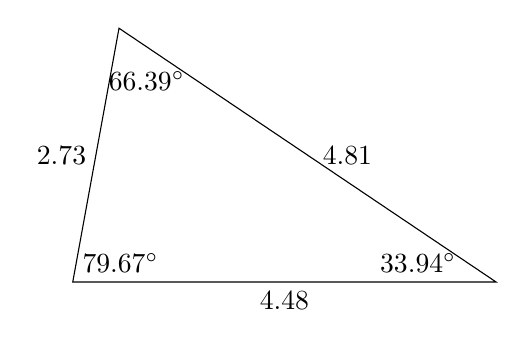
\begin{tikzpicture}[scale=1.2]
\coordinate (A1) at (0,0);
\coordinate (B1) at (4.48cm,0);
\coordinate (C1) at (79.67:2.73cm);
\node[above right] at (A1) {$79.67^\circ$};
\node[above left,xshift=-11pt] at (B1) {$33.94^\circ$};
\node[below,yshift=-12pt,xshift=10pt] at (C1) {$66.39^\circ$};
\draw (B1) -- node[below] {$4.48$} (A1) --
  node[left] {$2.73$} (C1) -- node[right,xshift=2pt] {$4.81$} cycle;
\end{tikzpicture}
\end{center}
\caption{Das Dreieck mit demselben Umfang und derselben Fläche wie $(3,4,5)$}\label{f.not-a-right-triangle}
\end{figure}

\subsection*{Was ist die Überraschung?}

Sind Dreiecke mit gleichem Flächeninhalt und Umfang kongruent? Mein erster Eindruck war, ``Ja'' zu sagen, denn es ist nicht leicht, Gegenbeispiele zu finden. Überraschend ist, dass es bei einem beliebigen Dreieck mit rationalen Seiten möglich ist, ein nicht kongruentes Dreieck mit rationalen Seiten zu konstruieren, das denselben Flächeninhalt und Umfang hat, obwohl das Ergebnis seltsam sein kann, wie bei den Dreiecken $(3,4,5)$ und $\left(\frac{156}{35}, \frac{101}{21}, \frac{41}{15}\right)$.

\subsection*{Quellen}

Dieses Kapitel stützt sich auf \cite{mccallum}. In \cite{marita} wird gezeigt, dass es bei einem isozyklischen Dreieck nicht kongruente Dreiecke mit demselben Flächeninhalt und Umfang gibt, aber der Beweis enthält keine explizite Konstruktion.
